\providecommand{\toplevelprefix}{../..}  % necessary for subfile bibliography + figures compilation to work, do not move this after documentclass
\documentclass[../../book-main.tex]{subfiles}

\begin{document}

\chapter{Future Study of Intelligence}
\label{ch:future}

% \begin{quote}
% ``{\em If I were to choose a patron saint for cybernetics
% out of the history of science, I should have to choose
% Leibniz. The philosophy of Leibniz centers about two
% closely related concepts -- that of a universal symbolism
% and that of a calculus of reasoning.}''

% $~$\hfill -- Norbert Wiener, Cybernetics, 1961
  
% \end{quote}

\begin{quote}
``{\em The study is to proceed on the basis of the conjecture that every aspect of learning or any other feature of intelligence can in principle be so precisely described that a machine can be made to simulate it. An attempt will be made to find how to make machines use language, form abstractions and concepts, solve kinds of problem now reserved for humans, and improve themselves.}''

$~$\hfill -- Proposal for the Dartmouth AI program, 1956
 \end{quote}
\vspace{5mm}

%This chapter discusses active ongoing research topics on intelligence as well as some challenges and opportunities for future study.

Generally speaking, this manuscript is meant to systematically introduce mathematical principles and computational mechanisms for how memory or knowledge can be developed from empirical observations. The capability to seek parsimony in a seemingly random world is a fundamental characteristic of any intelligence, natural or man-made. We believe that the principles and mechanisms presented in this book are rather unifying and universal and are applicable to both animals and machines. 

We hope that this book can help the readers fully clarify the mystery around modern practices of artificial deep neural networks by developing a rigorous understanding of their functions and roles in achieving the objective of learning low-dimensional distributions from high-dimensional data. With such a understanding, we should have become rather clear both capabilities and limitations of existing AI models and systems: 
\begin{enumerate}
    \item Existing models and systems are short of being complete in terms of a memory system that is capable of self-learning and self-improving.
    \item Existing realizations of these functions are still rather primitive and brute force and certainly far from optimal in terms of optimization strategies hence network architectures. 
    \item Existing AI models only learn the data distribution and conduct inductive (Bayesian) inference, which is different from the high-level human intelligence.
\end{enumerate} 

One of the goals of this book is for people to establish an objective and systematic understanding of current machine intelligence technologies and to realize what open problems and challenges remain ahead for further advancement of machine intelligence. In the last chapter of the book, we provide some of our views and projections for the future. 

\section{Towards Autonomous Intelligence: Close the Loop?}
From the practice of machine intelligence in the past decade, it has become clear that, if there were sufficient data and computational resources, one could build a large enough model and pre-train it to learn the {\em a priori} distribution of all the data, say $p(\x)$. Theoretically, such a large model can memorize almost all existing knowledge about the world that has been encoded in massive languages and texts. As we have discussed at the beginning of the book, in a way, such a large model plays a similar role as DNAs with which life uses to record and pass on knowledge about the world.  

The so learned model and distribution can then be used to regenerate new data samples based on the same distribution. One can also use the model to conduct inference (e.g., estimation, prediction) with the memorized knowledge under various conditions, say by sampling the {\em a posteriori} distribution $p(\x\mid \y)$ under a new observation $\y$. Strictly speaking, such inference is statistical. 

Any pre-trained model, however large, cannot guarantee that the distribution that it has learned so far is entirely correct or complete. In case our samples  $\hat{\x}_t$ from the current {\em a priori} $p_t(\x)$ or estimates $\hat{\x}_t(\y)$ based on the {\em a posteriori} $p_t(\x\mid \y)$ are inconsistent with the truth $\x$, we would very much like to correct the learned distributions:
\begin{equation}
    p_t(\x) \rightarrow p_{t+1}(\x) \quad \mbox{or}\quad p_t(\x\mid \y) \rightarrow p_{t+1}(\x\mid \y),
\end{equation}
based on the error $\boldsymbol{e}_t = \x_t - \hat{\x}_t$. This is known as error correction based on error feedback, an ubiquitous mechanism in nature for continuous learning. However, as we know, any open-ended model itself does not have the mechanisms to revise or improve the learned distribution when it is incorrect or incomplete. Improving current AI models still largely depends on human involvement: experimentation, evaluation, and selection. We may call this process as ``artificial selection'' of large models, as opposed to the natural selection for the evolution of lives. 

As we have studied earlier in this book (Chapter \ref{ch:closed-loop} in particular), closed-loop systems allows to align an internal representation with the (sensed) observations of the external world. It can continue to improve the internally learned distribution and its representation to achieve consistency or self-consistency. An immediate step forward for the future is to develop and build truly closed-loop memory systems, as shown in Figure \ref{fig:open-to-closed}, that are capable of learning and improving more general data distributions autonomously and continuously based on error feedback. 

Therefore, transition from the current popular end-to-end trained open-loop models to continuously-learning closed-loop systems:
\begin{equation}
   \mbox{\textbf{open-ended} models} \; \Longrightarrow \; 
   \mbox{\textbf{closed-loop} systems}
\end{equation}
is the key for machines to truly emulate how the (animal) brain learns and applies knowledge in an open world. We believe that
\begin{quote}
\begin{center}
        {\em open-ended models are for a closed world, however large; \\ closed-loop systems are for an open world, however small.}
\end{center}
\end{quote}
In fact, ``general intelligence'' could never be achieved by simply having memorized all existing knowledge of the world. Instead, general intelligence can only be achieved by having the mechanisms to improve its existing memory so as to be able to adapt to any new environments and tasks. 

\begin{figure}[t]
    \centering    
    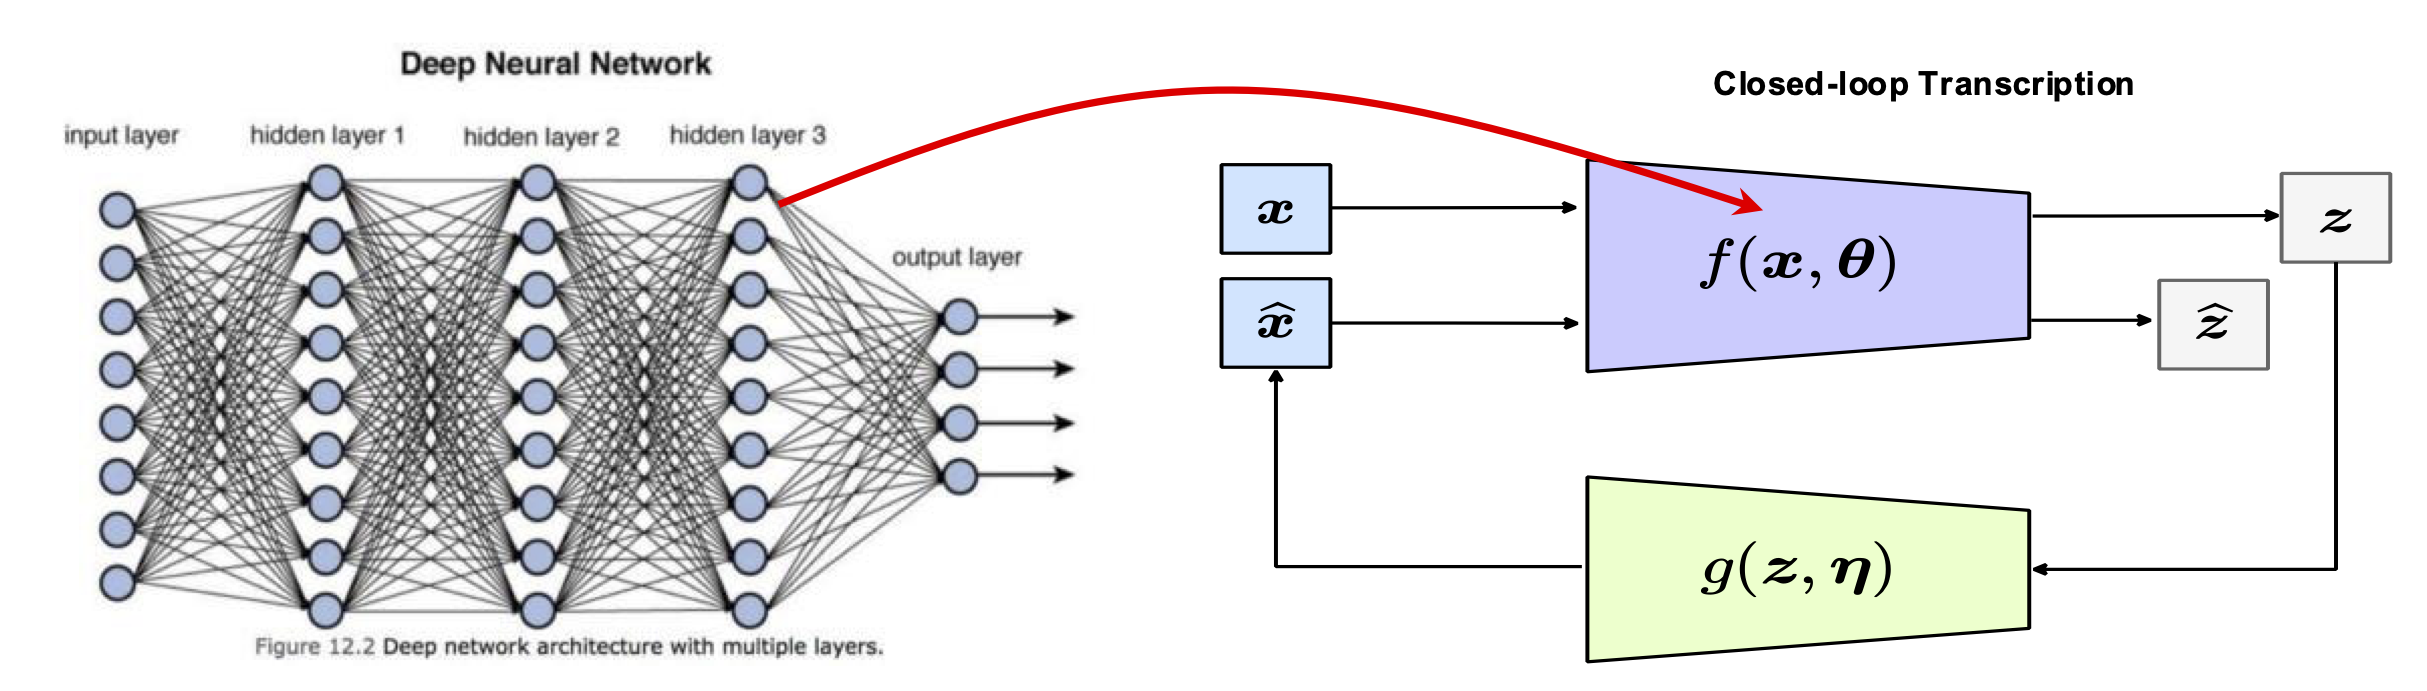
\includegraphics[width=0.9\linewidth]{\toplevelprefix/chapters/chapter8/figs/open-to-closed.png}
    \caption{From an open-ended deep network to a closed-loop system.}
    \label{fig:open-to-closed}
\end{figure}



\section{Towards Intelligence of Nature: Beyond Back Propagation?}
The practice of machine intelligence in the past few years has led many to believe that one needs to build a single large model to learn the distribution of all data and memorize all knowledge. Even if this might be technologically possible, it is likely that such a solution is far from necessary and efficient. As we have known from the practice of training deep networks, the only known scalable method to train such networks at scale is through back propagation (BP) \cite{Back-Prop}. Although BP has offered a way to correct errors via gradient signals propagated back through the whole model, it is nevertheless rather brute force and differs significantly from how nature learns: BP is an option that nature cannot afford in terms of its high cost or simply cannot implement due to physical limitations. 

More generally, we cannot truly understand intelligence unless we also understand how it can be efficiently implemented. That is, one needs to address the computational complexity of realizing mechanisms associated with achieving the objectives of intelligence. Note that, historically, our understanding of (machine) intelligence has precisely evolved through several phases, from the incomputable Kolmogorov complexity to Shannon's entropy, from Turing's computability to later understanding of  tractability,\footnote{We say a problem is tractable if it allows an algorithm whose complexity is polynomial in the size of the problem.} and to the strong emphasis on algorithm scalability in modern practice of artificial intelligence. This evolution can be summarized as the following diagram:
\begin{equation}
   \mbox{\textbf{incomputable}} \;
   \Longrightarrow \; \mbox{\textbf{computable}} \;
   \Longrightarrow \; \mbox{\textbf{tractable}} \; \Longrightarrow \; 
   \mbox{\textbf{scalable}}.
\end{equation}
To a large extent, the success and popularity of deep learning and back propagation is precisely because they have offered a  scalable implementation with modern computing platforms (such as GPUs) for processing and compressing massive data. Nevertheless, such an implementation is still way too more expensive compared to how nature realizes intelligence. 

There remains a huge room for  improvement of the efficiency of   machine intelligence so that it can emulate the level of efficiency of natural intelligence, which should be of magnitudes more efficient than the current brute-force implementations. To this end, we need to discover new learning architectures and optimization mechanisms that enable learning data distributions under natural physical conditions and resource constraints, similar to those for intelligent beings in nature, say, without accessing all data at once or updating all model parameters (by BP) at once. 

The principled framework and approach laid out in this book can guide us to discover such new architectures and mechanisms.  These new architectures and mechanisms should enable online continuous learning and can be updated through highly localized and sparse forward or backward optimization. So far, for learning a distribution, the only case for which we know such a solution exists is the simplest case of PCA, with the online PCA method introduced in Chapter \ref{ch:autoencoding}.  

\begin{figure}[t]
\centering
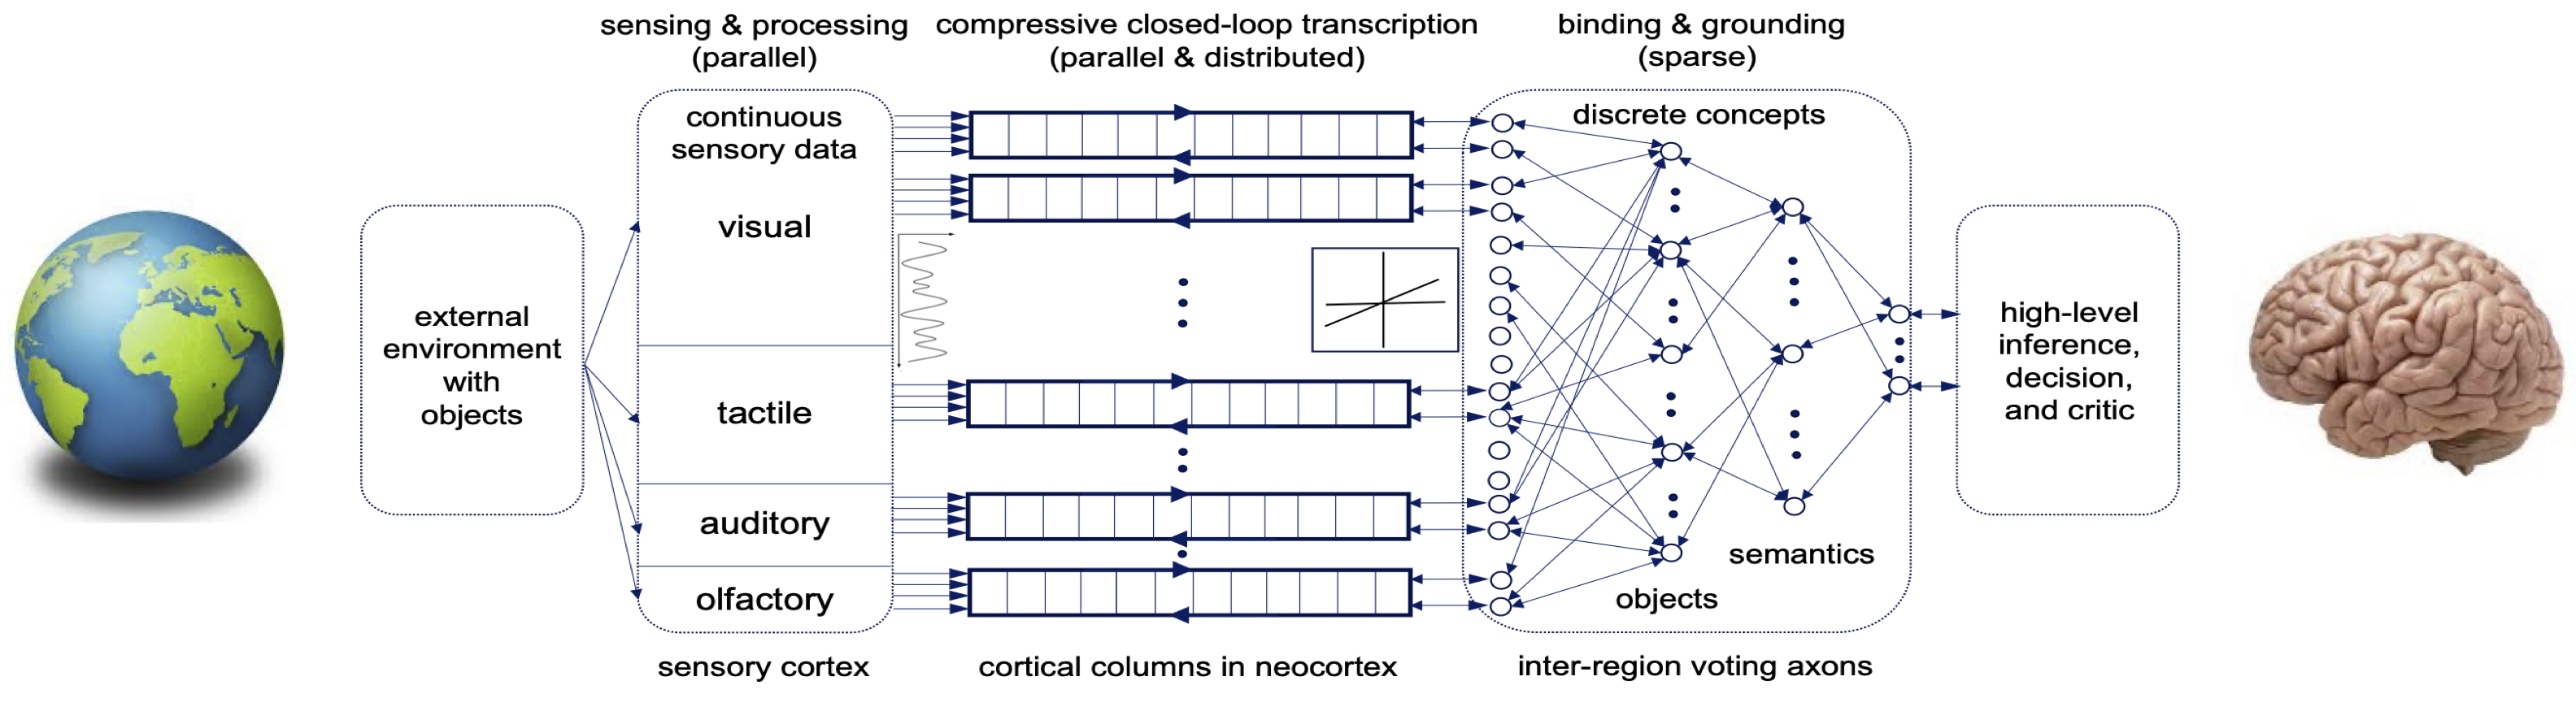
\includegraphics[width=0.99\linewidth]{\toplevelprefix/chapters/chapter8/figs/loops.png}
    \caption{Conjectured architecture of the brain cortex: The cortex is a massively parallel and distributed auto-encoding system that consists of a hierarchy of closed-loop auto-encoders that extract information from multiple senses and maximize the information  gain of the resulting representations at multiple levels of hierarchy and granularity.}
    \label{fig:loops}
\end{figure}
As we have learned from neuroscience, the cortex of our brain consists of tens of thousands of cortical columns. All cortical columns have similar physical structures and functions. They are highly parallel and distributed, though sparsely interconnected. Hence, we believe that in order to develop a more scalable and structured memory system, we need to consider architectures that emulate that of the cortex. Figure \ref{fig:loops} shows such a hypothesized architecture, a massively distributed and hierarchical system that consists of many largely parallel closed-loop auto-encoding modules. These modules learn to encode different sensory modalities or many projections of data from each sensory modality. Our discussion in Section \ref{sec:measurement-self-consistency} of Chapter \ref{ch:conditional-inference} suggests that such a parallel sensing and learning of a low-dimensional distribution is theoretically possible. Higher-level (lossy) autoencoders can then be learned based on outputs of lower-level ones to develop more sparse and higher-level  ``abstractions'' of the representations learned by the lower levels. 


The distributed, hierarchical, and closed-loop system architecture illustrated in Figure \ref{fig:loops} shares many characteristics of cortex of the brain. Such a system architecture may open up many more possibilities than the current single large-model architecture. It makes exploring much more efficient learning and optimization mechanisms possible, and resulting more structured modular organization of the learned data distribution and knowledge. This would allow us to bring the implementation of machine intelligence to the next level of evolution: 
\begin{equation}
   \mbox{\textbf{incomputable}} \;
   \Longrightarrow \; \mbox{\textbf{computable}} \;
   \Longrightarrow \; \mbox{\textbf{tractable}} \; \Longrightarrow \; 
   \mbox{\textbf{scalable}} \; \Longrightarrow \; 
   \mbox{\textbf{natural}}.
\end{equation}

\section{Towards Intelligence of Human: Beyond the Turing Test?}
As we have discussed at the beginning of this book, Chapter \ref{ch:intro}, intelligence in nature has evolved through multiple phases and manifested in four different forms:
\begin{equation}
\mbox{\textbf{phylogentic}} \;
   \Longrightarrow \; \mbox{\textbf{ontogenetic}} \; \Longrightarrow \; 
   \mbox{\textbf{societal}}
   \; \Longrightarrow \; 
   \mbox{\textbf{artificial intelligence}}.
\end{equation}
All forms of intelligence share the common objective of learning useful knowledge as certain low-dimensional distributions of sensed high-dimensional data about the world. However, they may differ significantly in the specific coding schemes adopted, the information encoded, computational mechanisms for learning and improving, and physical implementations of such mechanisms. Using the concepts and terminologies developed in this book, from the perspective of learning and representing information or knowledge from the distribution of the sensed data, the above four stages of intelligence developed in nature differ in the following three aspects:
\begin{itemize}
    \item The codebook that one uses to learn and encode the intended information or knowledge.
    \item The information or knowledge that are encoded and represented using the codebook. 
    \item The optimization mechanisms used to improve the information or knowledge encoded.
\end{itemize}
More specifically, the following table summarizes their main characteristics in the above three aspects:
\begin{center}
%\begin{small}
\begin{tabular}{| c | c | c | c | c |}
\hline & \textbf{Phylogentic} & \textbf{Ontogenetic} & \textbf{Societal} & \textbf{Artificial}\\
\hline
\textbf{Codebook}  & Amino Acids & Neurons & Alphabet \& Words & Mathematics/Logic \\ [0.5ex]
  \hline 
\textbf{Information} & Genes/DNAs & Memory & Languages/Texts & Scientific Facts\\ [0.5ex]
  \hline
\textbf{Optimization} & Reinforce Learning & Error Feedback & Trial \& Error & Hypothesis Testing \\  [0.5ex]
\hline
\end{tabular}
%\end{small}
\end{center}


% \begin{equation}
% \mbox{\textbf{Amino Acids}} \;
%    \Longrightarrow \; \mbox{\textbf{Brain}} \; \Longrightarrow \; 
%    \mbox{\textbf{Languages}}
%    \; \Longrightarrow \; 
%    \mbox{\textbf{Mathematics \& Logic}}.
% \end{equation}

% \begin{equation}
% \mbox{\textbf{Genes}} \;
%    \Longrightarrow \; \mbox{\textbf{Memory}} \; \Longrightarrow \; 
%    \mbox{\textbf{Books}}
%    \; \Longrightarrow \; 
%    \mbox{\textbf{Science}}.
% \end{equation}

% \begin{equation}
% \mbox{\textbf{RL}} \;
%    \Longrightarrow \; \mbox{\textbf{Feedback}} \; \Longrightarrow \; 
%    \mbox{\textbf{Empirical}}
%    \; \Longrightarrow \; 
%    \mbox{\textbf{Hypotheses Testing}}.
% \end{equation}


As we now know, humans have achieved two quantum leaps in intelligence in history.
The first is the development of spoken and written languages about five to ten thousand years ago. That has enabled human to share and pass on learned knowledge for generations, similar to the role of DNAs in nature. The second is the development of mathematics and logic about three thousand years ago, which have become a precise language for modern science. This new language has freed us from summarizing knowledge from observations in empirical forms and allowed us to formalize knowledge as verifiable or falsifiable theories either through mathematical deduction or experimental verification. Through hypothesis formulating, logic deduction, and experimental testing, we are able to proactively discover new knowledge that was previously impossible by passively learning from data distribution.\footnote{such as causal relationships}

As we have discussed in the Introduction (Chapter \ref{ch:intro}), the 1956 ``artificial intelligence'' (AI) program precisely aimed to study high-level functions such as mathematical abstractions, logical inference, and problem solving that are believed to differentiate humans from animals: 
\begin{equation}
   \mbox{\textbf{low-level} (animal) intelligence} \; \Longrightarrow \; 
   \mbox{\textbf{high-level} (human) intelligence.}
\end{equation}
As we have clarified repeatedly in this book, much of the technological advances in machine intelligence in the past decades, although carried out under the name ``AI'', is actually more closely related to the low-level intelligence shared by both animals and humans, which is mainly inductive. So far, there has been no evidence suggesting that these mechanisms alone would suffice to achieve high-level human intelligence that the original AI program truly aims to understand and emulate. 

In fact, we know little about how to rigorously verify whether a system is truly capable of certain high-level intelligence, despite the fact that the Turing test has been proposed since 1950 \cite{Turing-1950}.\footnote{In Turning's proposal, the evaluator is a human. However, most human evaluators' scientific training and knowledge can be limited and their conclusions can be subjective.} For long such a test was not deemed necessary since the capabilities of machines were far below that of a human (or even animal). However, given recent technological advances, many models and systems have claimed to reach and even surpass human intelligence. Therefore, it is high time to give a scientific and executable definition of the Turing test. That is, how do we systematically and objectively evaluate the level of intelligence for a given model or system? For example, how can we rigorously verify whether an intelligent system has truly grasped a certain abstraction concept, such as the notion of natural numbers, or it has merely memorized a large number of instances? Note that the state-of-the-art large language models still struggle with simple mathematical questions like: ``Whether 3.11 is larger or smaller than 3.9?''\footnote{Note that some  models have corrected their answers to questions of this kind via post engineering. Or some models have incorporated additional reasoning mechanisms based on verifying the immediate answers produced and correct them during reasoning. However, we leave it to the reader as an exercise to rigorously test whether any of the state-of-the-art language models truly understand the notion of numbers (natural, rational, real, and complex) and the associated arithmetic.} 
How to verify whether a system truly understands the rules of logic and knows how to apply them rigorously or has simply memorized a large number of instances of practicing logic? Furthermore, is such a system even capable of correcting its own knowledge or developing new knowledge such as physical laws, mathematical concepts, or causal relationships? In summary, it is high time that we develop rigorous evaluation methods that can tell a system/model's seemingly intelligent capability belongs to which of the following: 
\begin{enumerate}
    \item simply having memorized the distribution of some knowledge-carrying data and regenerating them;
    \item being able to autonomously and continuously develop new knowledge from new observations;
    \item truly having understood certain abstract knowledge and knowing how to apply it correctly;
    \item being able to generate new scientific hypotheses or mathematical conjectures and verify them.
\end{enumerate}

\begin{figure}[t]
    \centering
    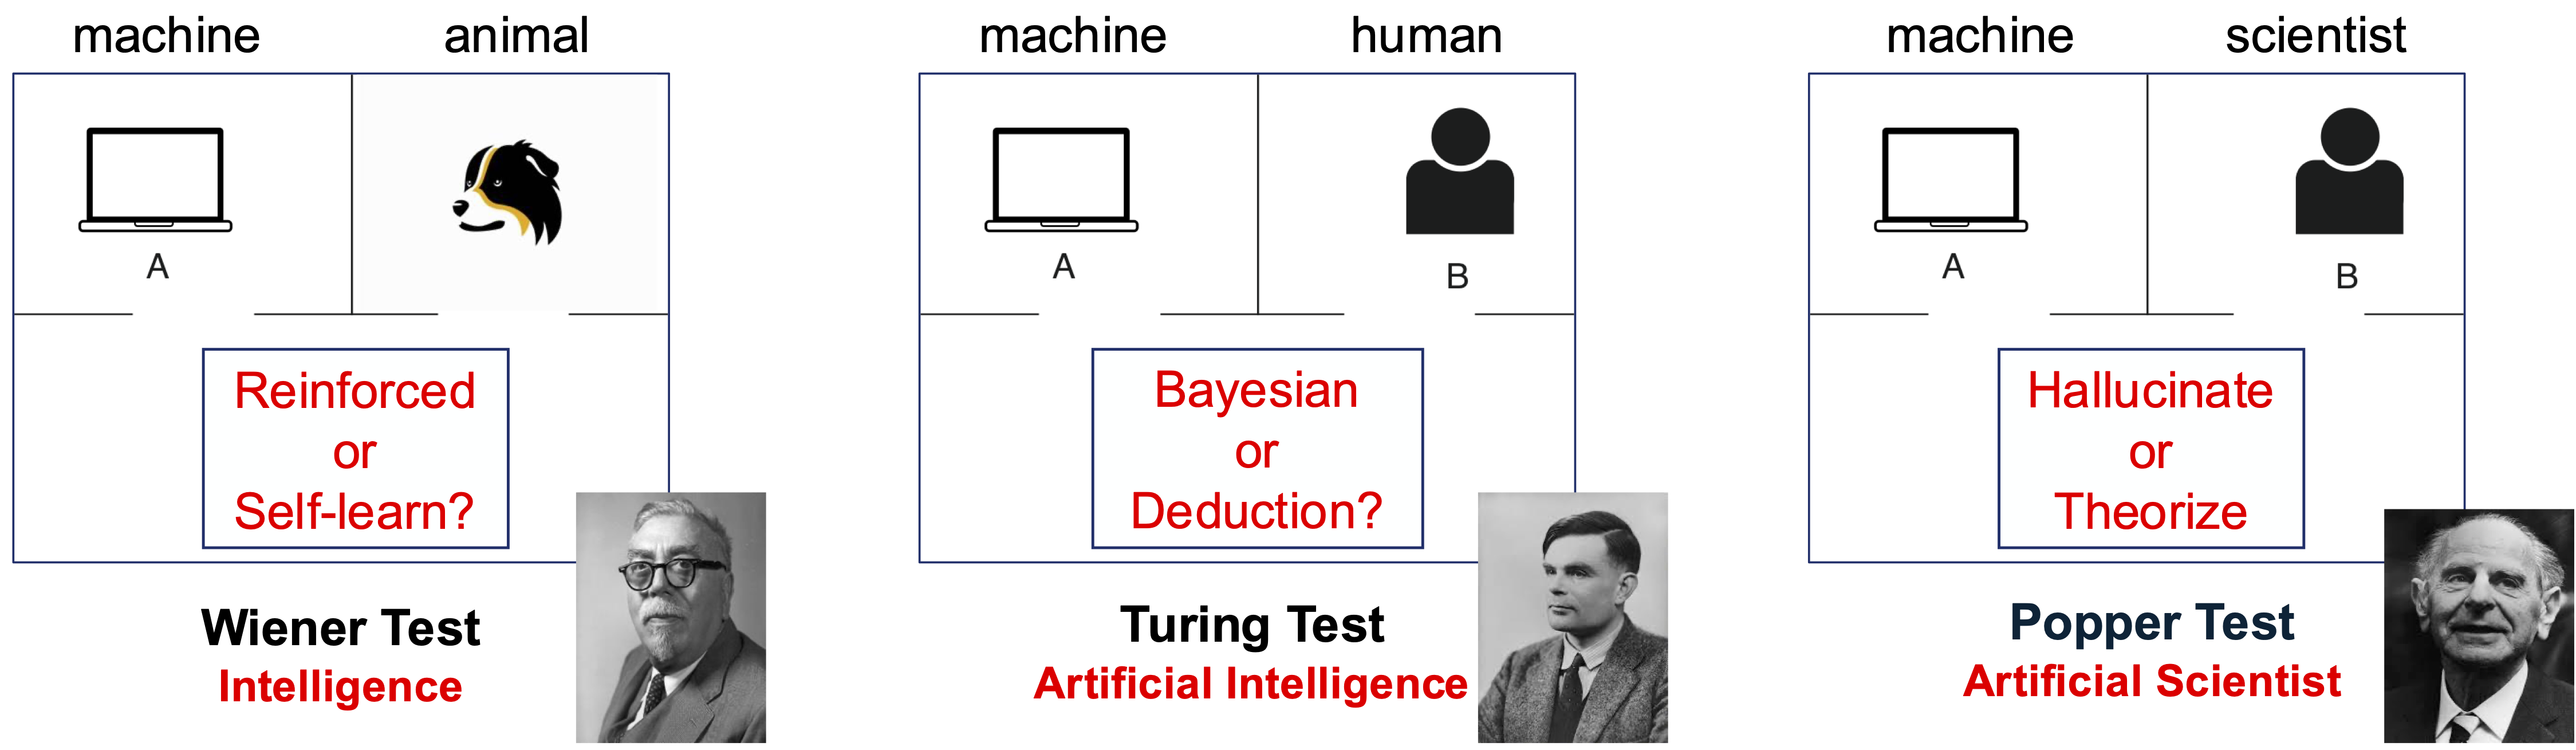
\includegraphics[width=0.95\linewidth]{\toplevelprefix/chapters/chapter8/figs/tests.png}
    \caption{Three tests for different levels or types of intelligence capabilities: the Wiener test, the Turing test, and the Popper test.}
    \label{fig:three-tests}
\end{figure}

Figure \ref{fig:three-tests} illustrate that probably there should be at least three different types of tests to evaluate and differentiate different types of intelligence capabilities:
\begin{enumerate}
    \item {\em The Norbert Wiener Test:} The evaluate whether a system is capable of improving and developing new knowledge of its own or simply receives information through reinforced or supervised learning;
    \item {\em The Alan Turning Test:} The evaluate whether a system can understand abstract knowledge or simply learns its statistics and uses it for Bayesian inference.
    \item {\em The Karl Popper Test:} To evaluate whether a system is capable of exploring new knowledge through forming and verifying new theories based on self-consistency.
\end{enumerate}
We believe that, for such evaluation methods, the evaluator should not be a human but a scientifically sound protocol and process, instead.



As we have seen throughout this entire book, {\em compression} has played a most fundamental role in learning. It is the governing principle and a unified mechanism for identifying an (empirical) data distribution and organizing information encoded therein. To a large extent, it explains most of the practice of ``artificial intelligence'' in the past decade or so. Here the word ``artificial'' largely means ``man-made.'' An outstanding question for future study is whether {\em compression alone} is sufficient to achieve all higher-level capabilities of intelligence listed above? 
\begin{quote}
\begin{center}
        {\em Is compression all there is?}
\end{center}
\end{quote}
Whether abstraction, causal inference, logical reasoning, and hypothesis generating and the subsequent deduction are certain extended or extreme forms of compression? Is there a fundamental difference between identifying  empirical) data distributions through compression and extracting high-level theories or laws? Philosopher Sir Karl Popper has once suggested:
\begin{quote}
    \begin{center}
    {\em ``Science may be described as the art of systematic oversimplification.''}
    \end{center}
\end{quote}
To a large extent, Science can be viewed as the most advanced form of intelligence, hence the true ``artificial'' part of our intelligence. Here the word ``artificial'' means what is unique to the enlightened humans, almost like a form of high art. We believe that uncovering and understanding the underlying mathematical principles and computational mechanisms of such higher-level intelligence will be the final frontier for Science, Mathematics, and Computation altogether!

\end{document}